\documentclass[conference]{IEEEtran}
\IEEEoverridecommandlockouts
% The preceding line is only needed to identify funding in the first footnote. If that is unneeded, please comment it out.
\usepackage{cite}
\usepackage{amsmath,amssymb,amsfonts}
\usepackage{algorithmic}
\usepackage{graphicx}
\usepackage{textcomp}
\usepackage{xcolor}
\usepackage{csquotes}
\usepackage[T1]{fontenc}
\usepackage{listings}
\lstset{
  frame=single,
  breaklines=true,
  numbers=left,
  numbersep=3pt,
  numberstyle=\small,
  language=python,
  tabsize=2,
  showstringspaces=false,
  upquote=true,
}
\renewcommand{\lstlistingname}{Code}

\def\BibTeX{{\rm B\kern-.05em{\sc i\kern-.025em b}\kern-.08em
    T\kern-.1667em\lower.7ex\hbox{E}\kern-.125emX}}
\begin{document}
\title{A New Feature to Secure Web Applications}

\author{\IEEEauthorblockN{Kohei Kubota}
\IEEEauthorblockA{\textit{ISEE. Kyushu University} \\
Fukuoka, Japan \\
kubota.kohei.474@s.kyushu-u.ac.jp}
\and
\IEEEauthorblockN{Wai Kyi Kyi Oo}
\IEEEauthorblockA{\textit{ISEE. Kyushu University} \\
Fukuoka, Japan \\
kyi.oo.wai.kyi.219@s.kyushu-u.ac.jp}
\and
\IEEEauthorblockN{Hiroshi Koide}
\IEEEauthorblockA{\textit{RIIT. Kyushu University} \\
Fukuoka, Japan \\
koide@cc.kyushu-u.ac.jp}
}

\maketitle

\begin{abstract}
Web application security is one of essential components of any web-based systems.
As becoming popular of the Internet makes many web sites be attacked by many kinds of  attacks.
So, we have to propose a secure framework for web applications.
For this reason, we have to propose a web application framework which not only analyzes the source code implemented by web developers, also it can detects the vulnerabilities in the source code dynamically.
Although a lot of research works have already proposed detection methods of vulnerabilities in web application attacks, but those are not fully detected because their methods do not use the information of the web applications.
Therefore, we propose a new method which analyzes the source code of a web application, and then modifies it if needed, in addition, our method has a detection method of an application ’s vulnerabilities that are difficult to detect by previous methods.
According to our implementation and experiments, it is possible to detect actual attacks, which have been considered difficult to detect, against authentication leaks and SQL injection attacks using dynamic queries.
\end{abstract}

\begin{IEEEkeywords}
web security, web application framework, secure programing
\end{IEEEkeywords}

\section{Introduction}
Web application security has been an important topic when it comes to the security field.
As the growth of the Internet exposes any web-based system to attacks from different locations and various levels of complexity.
Web application security deals specifically with the websites, web applications and web services such as application programming interfaces (API).
With the aim of improving security functions or methods of web application frameworks, we propose an effective framework which has features of analyzing callback functions, and it can modify the source code of an application in case it needs to be changed.
Almost all web application frameworks provide application developers extensive functions to improve security of web applications.
By using these extensive functions of web application frameworks properly, application developers can develop secure applications efficiently.
However, developers using web application frameworks sometimes implement vulnerable applications, because not all developers can not use these extensive functions of web application framework properly.
In addition, web application frameworks do not analyze and modify callback functions that developers implement.
Thus, once a vulnerable application is created, it remains vulnerable until it is fixed.

Some web application frameworks provide developers unit test tools.
Using these tools, application developers could analyze their callback functions dynamically.
However application developers must describe various test data, which increase development time and workload, and it is difficult to describe test data for each vulnerability.

A method to reduce the vulnerability in web applications is to use web application firewall (WAF)\cite{kruegel2003anomaly, epp2017anomaly, makiou2014improving, krueger2010tokdoc, ito2018web}.
WAF is a system to protect web applications from vulnerable attacks like cross site scripting (XSS)\cite{subramaniyaswamy2018securing} or SQL injection (SQLi)\cite{halfond2005amnesia}.
WAF is usually placed between the client and the web application.
WAF receives requests from clients and verify requests whether the incoming requests are attacks or not.
If WAF detects an attack request, the request is blocked or sanitized.
WAF can reduce vulnerable attacks without modifying web applications and is especially effective in situations where the application cannot be modified directly.
On the other hand, WAF is not a fundamental solution to defense in implementation because WAF does not consider the status of applications and does not modify applications.
Eventually, it is necessary to modify applications for the fundamental countermeasure of attacks.
In addition, there are some attacks that are hard to detect using WAF.
WAF usually detects attacks using special characters in a request.
Thus, vulnerability attacks in terms of authentications and authorizations are difficult to protect using WAF,  since they can be carried out without the use of special characters.

%proposed method
In order to solve these problems, we propose a web application framework which has a feature of analyzing source code.
Our framework can be able to analyze the source code implemented by web application developers.
When an application is executed, our framework analyze callback functions and detect the vulnerable part of the callback functions.
Vulnerable source code is detected, this framework inserts functions to secure the source code or replaces the source code with secure one.
By using our proposed framework, web application developers can verify their application dynamically without additional implementation for vulnerability analysis.
In addition, our proposed framework can prevent vulnerability attacks, which is difficult to take measures with general web application frameworks and WAFs,  like authentication leak.

%implementation
Our framework modifies callback functions in four steps.
First, it gets the source code of callback functions from functions which are live objects.
Second, it then creates abstract syntax tress based on these callback functions.
In the third stage, it modifies created abstract syntax trees. In this stage, we use vulnerability handling functions implemented by the framework developers in order to modify the abstract syntax trees.
Finally, our framework makes live callback functions from the modified abstract syntax trees.
In these four steps, the application framework modifies the callback functions, and then these functions will be stored in our framework.
In order to prove whether our framework can verify the callback functions using vulnerability handling functions, we conducted experiments and analysis.

According to the results, we find that our framework is able to modify the measures against two vulnerabilities, the authentication leaks and SQL injection vulnerability.

% structure of this paper
The paper is organized as follows:
In section 2, we describe background about web application security, especially automatic defense method.
We take web application framework and WAF as an example.
In section 3, we introduce a web application framework.
In section 4, we describe how to implement the web application framework and an experiment in section 5.
In section 6, we describe about result of the experiment.
In section 7, conclusions are about the result.
\section{Background}
% webアプリケーションフレームワーク自動サニタイズ弱い
Web application frameworks\cite{chaudhuri2010symbolic} including many libraries can help developers in improving their applications efficiently.
Regarding security, web application frameworks provide security helper functions which are methods to secure callback functions or to add proper sanitization code to the web applications automatically, which is called auto-sanitization\cite{weinberger2011systematic}.
Security helper functions can hide complexities from application developers.
These security helper functions allow web application developers to efficiently develop secure applications.
However, web application developers need to call security helpers properly, which we have seen is an error-prone requirement.
Auto-sanitization is a feature that delegates some of the security overhead from application developers to the web application framework.
Web application developers indicate variables to sanitize, and web application frameworks sanitize them properly.
The benefit of auto-sanitization is that web application developers do not need to implement correct sanitization.
In general auto-sanitization, web application developers are responsible for indicating the variables that need to be sanitized.
Thus, vulnerable web applications can be created due to failure to indicate proper variables.
In addition, many auto-sanitize is applied only to template processing.
This means that these auto-sanitize have limited vulnerabilities that can be reduced.

% (wafで対策しづらい攻撃) /admin_pageが一般的なリクエストとして利用されるなら、GET /admin_pageはwafで防御不可能
WAF protects a web application from malicious attacks.
WAF is placed between the clients and the web application server and inspects HTTP requests and decides whether the requests are attacks or not.
WAF reduces the impact of an attack by not sending the attack request to the web application.
When an attack is determined, the request is converted by WAF into a secure one and sent to the web application, or WAF provides an error page back to the client.
Normally, the request is the only factor for WAF to determine whether it is an attack.
The more special characters that characterize attacks in the request, the easier WAF can detect the attacks.
Thus, WAF has a high detection rate of attacks such as XSS and SQLi.
However, typical WAF cannot prevent attacks that have no special characters in the requests and is also used for normal communication.
One of the attacks is an attack aimed at lack of authorization control.
Authorization is to confirm whether a specific operation is permitted to the authenticated user.
Lack of authorization control is a vulnerability that allows a user who does not have the necessary privileges to perform a particular operation to perform that operation.

% WAFs can be classified into two types, depending on how the attack is identified; signature-based detection or anomaly-based detection.
% Signature-based detection is a method for determining whether an input value is an attack or not by using a signature that defines the pattern of an attack request.
% This method of detection has the disadvantage that signatures tend to be complicated to set up and difficult to set up where there are no pattern bypass attacks.
% Another detection method, anomaly-based detection, relies on a model of the intended behavior of users and applications, and deviations from this normal behavior are determined as attacks.

\section{Proposed Method}
In this section, we describe about our proposed web application framework that has a feature of modifying callback functions.
This framework has three advantages in perspective of  cybersecurity.
First, application developers do not need to implement some security functions in callback functions.
By using general web application frameworks, web application developers have full responsibilities for implementing secure callback functions.
Since our framework can modify callback functions, it is responsible for part of the cybersecurity in callback functions.
Second, our framework can countermeasure vulnerable attacks which can not be countered by WAF (Web Application Firewall).
Usually WAF can detect cyberattacks by inspecting features or traces that include in the contents of request messages, such as special characters and meaningful strings about other programing languages.
Therefore, it is difficult to prevent attacks from requests that do not include special characters and/or meaningful strings about other programing languages.
However our framework can deal with the vulnerable attacks which is caused by a vulnerability in callback functions if the framework implements a vulnerability handling function that modifies the vulnerability in callback functions.
For example, vulnerabilities which our framework can detect and WAF cannot detect are  authentication leaks.
These vulnerabilities are caused by web application developer’s careless.
These vulnerable attacks happen because privileged resources can be accessed without any privileges on resources in callback functions.
Our framework can prevent these attacks by searching privileges on resources from other callback functions and using them.
Third, our framework fixes callback functions, thus fundamentally removing these vulnerabilities.
WAF can not remove vulnerabilities in callback functions.
Therefore, even if countermeasures are taken for a certain attack request,  attacks that bypass WAF may be established.

When an application that uses our framework is executed, communication becomes possible through four steps.
Figure \ref{fig:4step} shows steps to modify callback functions.
%図2:必要なステップを図示。
\begin{figure*}[htbp]
\centering{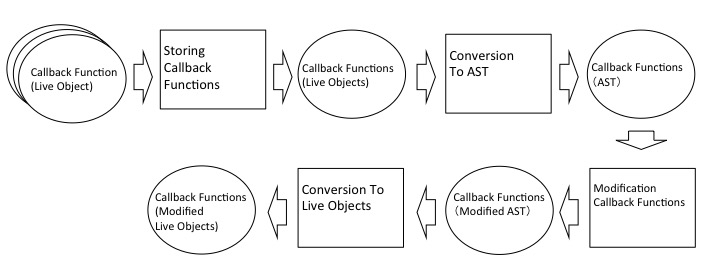
\includegraphics[bb=0 0 720 274, width=170mm]{./diagrams/slide1.jpg}}
\caption{Steps to modify callback functions.}
\label{fig:4step}
\end{figure*}
First, our framework stores callback functions with the information needed for routing.
At the moment, the callback functions are live objects which are binary data.
Next, to process callback functions easily, our framework converts the stored callback functions from live objects to abstract syntax trees (AST).
An AST is an intermediate code obtained in the process of making a program executable binary code.
The components of AST are represented by nodes, and each element represents the code object of program.
Since each node in the AST has a meaningful name or attribute name, it is easier to modify than to directly parse and modify the binary.
Also, AST has the advantage that it is easier to modify rather than modifying the source code.
In our method, it is difficult for the Web application framework to take the source code as an argument and directly modify the source code, because the developer who implements the vulnerability handling function cannot directly see the callback function.
This is because detecting source code vulnerabilities from regular expression and other string patterns are not suitable for detecting vulnerabilities.
An AST is easy to parse and modify because nodes in AST are removed the parts that have no meaning for the code object from the source code.
There are also types which group operators that have similar code generation rules.
Third is the modification of the callback functions.
Web application framework developers implements functions that modifies the callback function.
In this paper, we use this functions which can handle vulnerability functions.
These functions recursively search the syntax tree of the callback function from the conditions of the vulnerable nodes based on the node attributes and node names, and detects vulnerable nodes.
Then these functions modify the vulnerable callback function nodes.
The list of callback functions is the argument of the vulnerability handling function.
This process makes it possible to check the conditions of other callback functions based on the conditions written in other callback functions.
Finally, by converting the modified AST back into a live object, it is possible to use modified callback functions to communicate with the client.

\section{Implementation}
In this section, we present the source code as examples of the framework, and then describe the implementation of our framework. We use Python version 3.7 to implement the framework.
In particular, we describe how to implement the four steps described in the proposed method section: storing callback functions, converting to the abstract syntax tree, modifying the callback function, and reconverting to the live object.
From this section, in order to distinguish the names of developers, we will precisely address an application developer who implemented an application, and a framework developer who implemented a web application framework.
Figure \ref{fig:implementation_schematic} shows our framework's implementation.
\begin{figure*}[htbp]
\centering{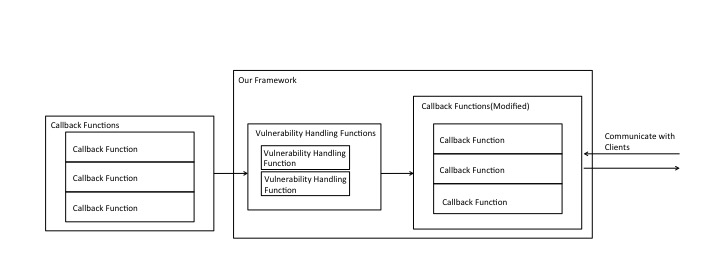
\includegraphics[bb=0 0 720 240, width=168mm]{./diagrams/slide3.jpg}}
\caption{Implementation schematic.}
\label{fig:implementation_schematic}
\end{figure*}

\subsection{Storing Callback Functions}
As a first step of implementation, our framework stores callback functions which is created by application developers.
The following source code is an example of writing a callback function(Code \ref{code:callback}).

\begin{lstlisting}[caption={An example of a callback function.}, label=code:callback, captionpos=b]
import app
@app.route(path='/', method='GET')
def index(request):
  return app.template("index.html")
\end{lstlisting}
The module we are importing in the first line(Code \ref{code:callback}) is our implementation of the web application framework.
This module provides the application developer with functions such as callback functions, routing and template functions, similar to general web application frameworks.
Regarding the second line(Code \ref{code:callback}), the route method stores index function implemented in the third line(Code \ref{code:callback}) and after in the web application framework.
The @ in the second line(Code \ref{code:callback}) is a description method called a decorator, and the following two source codes are equivalent expressions.

\begin{lstlisting}[caption={Python decorator.}, label=code:decorator, captionpos=b]
@decorator
  def func():
    ...
\end{lstlisting}

\begin{lstlisting}[caption={Source code synonymous with Code \ref{code:decorator2}.}, captionpos=b]
def func():
  ...
func = decorator(func)
\end{lstlisting}

%どのソースコードなの?
The route method receives three arguments, a path, a method, and a callback function.
In Code \ref{code:callback}, the path is `/', the method is `GET', and the callback function is index() function.
Then, the arguments become dictionary format, the path and the method as key, and the callback function as value.
This dictionary data is stored in the list as an element.
From above(Code \ref{code:callback}), the callback function is stored inside the framework and our framework is able to route based on paths and methods.

\subsection{Conversion to AST}
Next, we describe implementation that converts stored callback functions into an ASTs.

Since the callback functions stored in our framework are live objects and difficult to process, use the inspect module to obtain the source code for that objects.
The getsource method of inspect module takes an live object as an argument and returns its source code.
Live objects in Python have information such as function name and source code location.
By using that information, getsource method read a file and get the source code.
Note that this method does not have that information and will fail if the active object is created from exec or eval.
A generated AST becomes an dictionary format data which is composed a path and a method as key, and an the AST as value, and the dictionary format data is stored in a list as an element.

\subsection{Modification Callback Functions}
Third is modification.
Our framework uses the vulnerability handling function to modify callback functions of ASTs.
Figure \ref{fig:modification} shows how to modify callback functions by using vulnerability handling functions.
A vulnerability handling function receives the list.
Then the function parses and modifies the AST for each element, and returns modified list.
% 図に示すような感じで脆弱性ハンドリング関数の引数から修正され続ける図
\begin{figure*}[htbp]
\centering{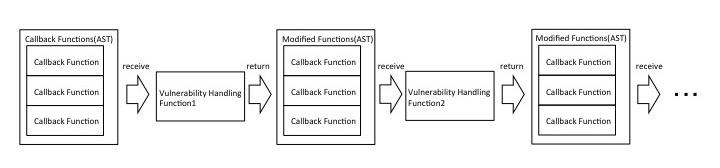
\includegraphics[bb=0 0 720 168, width=168mm]{./diagrams/slide4.jpg}}
\caption{Modification callback functions.}
\label{fig:modification}
\end{figure*}
An example of the source code of the vulnerability handling function is shown below(Code \ref{code:handling-example}).
\begin{lstlisting}[caption={An example of a vulnerability handling function}, label=code:handling-example, captionpos=b]
@node_fixer.add
def modifier(ast_callbacks):
  new_ast_callbacks = []
    for ast_callback in ast_callbacks:
      node = ast_callback.get('ast')
      new_node = NodeRewriter().visit(node)
      new_ast_callbacks.append(make_new_callback(ast_callback, new_node=new_node))
  return new_ast_callbacks
\end{lstlisting}

The node\_fixer.add method in the first line(Code \ref{code:handling-example}) adds the vulnerability handling function to our framework.
By attaching this decorator to each vulnerability handling function, our framework can modify ASTs of the callback functions with each vulnerability handling functions.
The new\_ast\_callbacks variable on the third line(Code \ref{code:handling-example}) is a list for inserting the dictionary data of modified callback functions.
In the for loop after the 4th line(Code \ref{code:handling-example}), each element of the list, that is, the abstract syntax tree of each callback function, is modified.
The fifth line(Code \ref{code:handling-example}) extracts the AST from the dictionary data and the six line(Code \ref{code:handling-example}) modifies the AST.
The NodeRewriter class is a child class of the ast.NodeTranformer class of Python's built-in module, and the framework developers must implement the child class of ast.NodeTransformer and describe the conditions of vulnerable nodes and the nodes to be fixed.
The visit method recursively searches the callback function node.
Then modified callback function is assigned at line 7(Code \ref{code:handling-example}) and returned as the modified list.

\subsection{Conversion to Live Objects}
The ASTs are transformed into live objects using Python built-in exec function.
This function is used for the dynamic execution of a program that can either be a string or object code.
With this function, our framework converts the AST of each element in the list into an execution object.

\section{Experiment}
We conducted experiments for each vulnerability by investigating whether the vulnerability handling function dynamically modified the callback function to reduce the impact of the vulnerabilities.
The vulnerable callback functions that were implemented in our framework were SQL injection and lack of authorization control.
We implemented vulnerability handling functions to modify each.
We conducted our experiment in the following environment; Mac OS X El Capitan 10.11.6, Intel Core i5 (2.95GHz), and main memory 8GB.
We carried out the execution of the application and attacks to the application locally.
%We executed in local.
First, it was confirmed whether the attack was affected by not implementing the vulnerability handling function, and then whether the handling function was implemented to reduce the impact of the attack.

In the following subsections, the callback function and the vulnerability handling function implemented for the experiment are shown, and the specific operation is described.

\subsection{Modify SQL Injection}
SQLi is a vulnerability that construct queries by directly using request parameters.
By inserted an invalid character string in the request parameter, the instruction not expected by the application developer is executed on SQL.
This causes tampering with the database and unauthorized deletion of data.
One of the measures of SQLi is to analyze SQL statements.

The following source code(Code \ref{code:sqli_callback}) has a SQLi vulnerability.
\begin{lstlisting}[caption={A vulnerable function which has a SQL injection.}, label=code:sqli_callback, captionpos=b]
@app.route("^/access$", "POST")
def access(request):
  import sqlite3
  conn = sqlite3.connect("test.sqlite3")
  cur = conn.cursor()
  action = request.forms.get('action')
  name = request.forms.get('name')
  password = request.forms.get('password')
  query = '{action} * from user'.format(action=action)
  if action='select':
    query += " where name = '{name}' and password = 'password'".format(name=name, password=password)
    cur.execute(query)
    data = cur.fetchone()
    return tmpl("access.html", action='select',tel=data[2],mail_address=data[3])
  else:
    cur.execute(query)
  return tmpl("access.html", action=action)
\end{lstlisting}
In the code above(Code \ref{code:sqli_callback}), the line 1 is the decorator that stores the callback function in the framework, the subsequent access function in the second line is the callback function which will be stored in the framework.
The argument named request of the access function is a dictionary data which stores the parameters of the request argument.
The preparations for creating SQL database is presented from line 3 to 5(Code \ref{code:sqli_callback}).
After that, from line 6 to 8(Code \ref{code:sqli_callback}), parameters are fetched from the request form, and these forms are used for building the SQL queries which are presented from line 9 to 11(Code \ref{code:sqli_callback}).
The variables we used in fetching from the request are ``action'', ``name'', and “password” from line 6 to 8(Code \ref{code:sqli_callback}). The “action” is the sql command, “name” is the username in the request, and “password” is the users’ password.
The cur.execute() method from line 13 to 15(Code \ref{code:sqli_callback}) will execute the queries which we extracted from the above variables in the database.
at line 10(Code \ref{code:sqli_callback}), we check the condition of variable “action”. If the action is ‘select’, cur.execute(query) at line 12(Code \ref{code:sqli_callback}) will be executed.
Next, at line 13(Code \ref{code:sqli_callback}), fetchone() method which is a built-in function of sqlite3 is implemented.
This method will return the result of executed queries in a tuple.
The returned result will be stored in a variable “data”. The third element of data is “phone number” and the fourth is “mail\_address”.
At line 14(Code \ref{code:sqli_callback}), this “access” calllback function uses a template method tmpl(), jinja2 template that will return elements which are “action”, “phone number”, and “email address” retrieved from the database to users.
As we can see that this source code is vulnerable, at lines 9 and 11(Code \ref{code:sqli_callback}), to the query which is created by directly using the request parameters.
Therefore, we can address this vulnerability with the following vulnerability handling function(Code \ref{sqli_handling}).

\begin{lstlisting}[caption={A vulnerable handling function which address a SQL injection.}, label=code:sqli_handling, captionpos=b]
@node_fixer.add
def insert_query_checker(ast_callbacks):
    new_ast_callbacks = []
    for ast_callback in ast_callbacks:
        node = ast_callback.get('ast')
        new_node = InsertQueryChecker().visit(node)
        new_ast_callbacks.append(make_new_callback(ast_callback, new_node=new_node))
    return new_ast_callbacks

class InsertQueryChecker(ast.NodeTransformer):
  def visit_Call(self, node):
    if isinstance(node.func, ast.Attribute):
      if isinstance(node.func.value, ast.Name):
        if node.func.value.id is 'cur':
          if node.func.attr is 'execute':
            new_args = []
              for arg in node.args:
                new_arg = ast.Call(
                  func=(ast.Name(id='escape_special_query', ctx=ast.Load())),
                    args=[arg],
                    keywords=[]
                  )
                new_args.append(new_arg)
                new_node = ast.Call(
                  func=node.func,
                  args=new_args,
                  keywords=node.keywords
                )
              return ast.copy_location(new_node, node)
    return node
\end{lstlisting}
To explain the above code(Code \ref{code:sqli_handling}), the vulnerability handling function which can modify the node is implemented from line 2 to 8.
The decorator on line 1(Code \ref{code:sqli_handling}) stores this function in our framework.
The class InsertQueryChecker searches and modifies the callback function node on line 6(Code \ref{code:sqli_handling}).
Then, visit\_Call() method is called when the node class name is Call which is a subclass of AST.
Nodes with the class name Call are function and method of nodes.
From line 14 to 16(Code \ref{code:sqli_handling}) describes the implementations of the node to be modified and their details.
The instruction is dropped and when “where” query is commented out in the select instruction.

\subsection{Modifying Lack of Authentication Control}
In this section, we show an example of a callback function which has an authorization control vulnerability.
\begin{lstlisting}[caption={A vulnerable function which has an authentication leak.}, label=code:auth_leak_callback, captionpos=b]
@app.route("^/login$", "POST")
def do_login(request):
    id = request.params["ID"]
    password = request.paramas["PASSWORD"]
    if is_admin(id, password):
        return "ADMIN_PAGE"
    else:
        return "LOGIN_PAGE"

@app.route("^/home$", "GET")
def home(request):
    return "ADMIN_PAGE"
\end{lstlisting}
The callback function named do\_login() takes request as an argument(Code \ref{code:auth_leak_callback}).
In order to return “ADMIN\_PAGE” to admin, it is required that id should be “admin” and password should be “admin\_pass”.
On the other hand, the path “/home” at line 10(Code \ref{code:auth_leak_callback}) is vulnerable in which all application users can see it.
To address this vulnerability, we implement the following source code(Code \ref{code:auth_leak_handling}).

\begin{lstlisting}[caption={A vulnerable function which address an authentication leak.}, label=code:auth_leak_handling, captionpos=b]
@node_fixer.add
def check_and_insert_is_admin(ast_callbacks):
  return_nodes_from_is_admin = []
  new_callbacks = []
  for ast_callback in ast_callbacks:
    node = ast_callback.get('ast')
    ret_node = search_return_node_from_if_auth_func(node=node, auth_func_name='is_admin')
    if ret_node:
      if len(return_nodes_from_is_admin) is 0:
        return_nodes_from_is_admin.append(ret_node)
      else:
        for n in return_nodes_from_is_admin:
          if ast.dump(n) is not ast.dump(ret_node):
              continue
          else:
            return_nodes_from_is_admin.append(ret_node)
            break
  for ast_callback in ast_callbacks:
    node = ast_callback.get("ast")
    ret_nodes = has_return_nodes(node, return_nodes_from_is_admin)
    if not ret_nodes:
      new_callbacks.append(ast_callback)
    else:
      new_node = None
      for ret_node in ret_nodes:
        if not from_is_admin(node, ret_node):
          new_node = InsertIsAdminFunc(ret_node).visit(node)
      new_callbacks.append(make_new_callback(ast_callback, new_node=new_node))
  return new_callbacks
\end{lstlisting}
The codes of “for” loop from line 5 to 16(Code \ref{code:auth_leak_handling}) find the node of the callback function that uses is\_admin() function which checks whether the admin or users.
This function is a helper function provided by the framework and returns “TRUE” if id and password are matched. Otherwise, it will return “FALSE”.
Callback function nodes that use this is\_admin() function are detected by line 7(Code \ref{code:auth_leak_handling}), search\_return\_node\_from\_if\_auth\_func() function and stored the result a list variable “return\_nodes\_from\_is\_admin”.
From line 18 to the rest of source code(Code \ref{code:auth_leak_handling}), the nodes stored in the list variable “return\_nodes\_from\_is\_admin” which are not authenticated by is\_admin() function will be changed to nodes which use is\_admin() function as an authenticated condition.

%In detail, 付録のnode\_fixer.pyを参照してください。

\section{Result}
As a result of the experiments, our framework was able to address the vulnerability in both experiments.
In the SQL injection countermeasure, the executed query is ``drop user;-where name =`name' and password =`pass' ''.
The user table was deleted when the vulnerability handling function was not implemented.
This query was not executed by sqlite3 when we implemented the handling function.

Next, regarding the lack of authorization control, ``ADMIN\_PAGE'' was returned when requesting ``/home'' with the browser when no countermeasure was taken.
On the other hand, when the vulnerability handling function was implemented, ``LOGIN \_PAGE'' was returned and we found that the countermeasure could be taken.

\section{Concluding Remark}
In this paper, as a function that the application should have, we proposed a function that automatically analyzes and modifies the callback function.
To evaluate our proposed framework and functions, we conducted experiments by implementing the web application and necessary steps.
From experiments and evaluations, we found that it is possible to partially deal with SQLi vulnerabilities and vulnerabilities with lack of authorization control.
On the other hand, it turns out that this framework has a challenge.
Since the vulnerability handling function must be implemented without implementing the callback function, it is difficult to implement the handling function.
To detect a wide range of vulnerabilities, it is necessary to increase the vulnerability handling functions.
We think that our framework can deal with a wide range of vulnerability by properly applying these functions to each callback function.
We believe that future improvements will make it easier to implement secure applications.

\section*{Acknowledgement}
This study is supported by Hitachi Systems.

\bibliography{IEEEabrv, ref.bib}
\bibliographystyle{IEEEtran}


\end{document}
